\title{Alocação de memória}
\frame{\maketitle}

\colorlet{textcolor}{brown!50!black}
\colorlet{initdatacolor}{green!30!black}
\colorlet{uninitdatacolor}{blue!30!black}
\colorlet{heapcolor}{red!70!black}
\colorlet{stackcolor}{cyan!30!black}


\begin{frame}{Introdução}

\begin{itemize}
\item \CEE\ fornece 4 rotinas de gerenciamento de memória: {\tt
malloc}, {\tt calloc}, {\tt realloc}, {\tt free}, que oferecem algumas
vantagens com relação a outros métodos de alocação:
\begin{itemize}
\item São padronizadas como parte da linguagem \CEE;
\item São mais fáceis de usar em programas com múltiplas {\it
threads};
\item Permite a alocação de pequenas unidades;
\item Permite a liberação de memória, que é mantida em uma lista livre
para ser utilizada posteriormente.
\end{itemize}

\item \bug{s} de gerenciamento de memória são comuns em \CEE, além de
serem difíceis de diagnosticar e reparar.
\end{itemize}
\end{frame}


\begin{frame}{Layout de memória de um processo no Linux}
  
\scriptsize

\begin{columns}
\begin{column}{.5\textwidth}
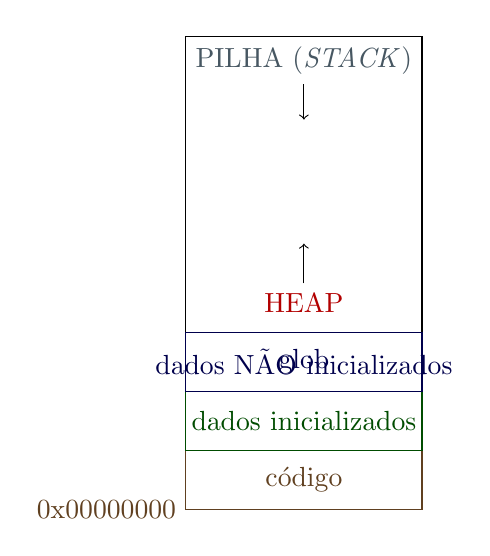
\begin{tikzpicture}

\def\D{3cm}
\def\H{2*\D}
\def\W{\D}
\def\CURH{0} % current height

\tikzset{
        every path/.style={->,draw},
        text/.style={textcolor},
        initdata/.style={initdatacolor},
        uninitdata/.style={uninitdatacolor},
        heap/.style={heapcolor},
        stack/.style={stackcolor},
        stackdata/.style={anchor=south,stackcolor,minimum width=\W,draw}
}
\draw (0,0) rectangle (\W,\H);
\def\CURH{\D/4}
\draw<1>[textcolor] (0,0) node[left] {0x00000000} rectangle node {código} (\W,\CURH);
\draw<1>[initdatacolor] (0,\CURH) rectangle node {dados inicializados}
(\W,2*\CURH);
\draw[uninitdatacolor] (0,2*\CURH) rectangle (\W,3*\CURH);
\node at (\W/2,2.5*\CURH) (unitdata position) {};
\node<1>[uninitdata]  at (unitdata position) {dados NÃO inicializados};
\node<2>[uninitdata] at (unitdata position) {glob};
\node<1>[heapcolor] at (2*\CURH,3.5*\CURH) (heap label) {HEAP};
\path<1> (heap label) -- +(0,\D/4);
% stack
\node<1>[stackcolor] at (\W/2,\H) (stack position) {};
\node<1>[stackcolor,below] at (stack position) (stack label) {PILHA ({\it STACK\/})};
\path<1> (stack label) -- +(0,-\D/4);
%\node<3>[stackdata] at (stack position) (stack int a) {a};
%\node<3>[stackdata] (stack int b) [below of=stack int a] {b};

\end{tikzpicture}
\end{column}
\begin{column}{.5\textwidth}
\begin{tabbing}
{\only<2>{\color{uninitdatacolor}}int glob;}\\

int \=soma(int x, int y) \{\\
    \>int s;\\
    \>s = x + y;\\
    \>return s;\\
\}\\
main(\=) \{\\
    \>int a, b;\\
    \>a = 3; b = 4;\\
    \>glob = soma(a,b);\\
\}\\
\end{tabbing}
\end{column}
\end{columns}

\end{frame}

\begin{frame}[fragile]{Protótipos}

\begin{lstlisting}

#include <stdlib.h> /* arquivo  de cabecalho a incluir */

/* aloca $size$ bytes e retorna um ponteiro 
   para a memoria alocada */
extern void *malloc(size_t size); 
/* libera o espaco de memoria apontado por $ptr$ */
extern void free(void *ptr);
/* aloca espaco para um vetor de $nmemb$ elementos 
   de tamanho $size$, e retorna um ponteiro para
   a memoria alocada */
extern void *calloc(size_t nmemb, size_t size);
/* muda o tamanho do espaco apontado por $ptr$
   para $size$ bytes, retornando um ponteiro para a 
   nova memoria alocada */
extern void *realloc(void *ptr, size_t size);
\end{lstlisting}

\end{frame}

\begin{frame}{malloc()}

\begin{tikzpicture}
\def\D{2cm}
\tikzset{
every path/.style={->,>=latex,draw},
decl/.style={draw},
chunk/.style={minimum width=1.5*\D, minimum height=\D/4,draw}
}

\node[anchor=west] at (0,0) (P) {\tt int *p;};
\node<2->[anchor=west] at (0,-\D/4) (M) {\tt p = malloc(nbytes);};
\node<3->[anchor=west] at (0,-\D/2) (dots) {$\ldots$};
\node<4>[anchor=west] at (0,-\D/1.5) (FREE) {\tt free(p);};

\node[decl] (Pdraw) [right of=P, xshift=\D, yshift=\D/2] {\tt \only<1,4>{\color{red}0x0}\only<2-3>{0xFF}};
\node<2->[anchor=west] [left of=Pdraw] {\it\small p};

\node<2,3>[chunk] (Mchunk) at (4*\D, -\D/8) {\it\color{gray} nbytes};
\node<2,3>[anchor=west] [left of=Mchunk,xshift=-\D/2] {\it\scriptsize 0xFF};

\path<1>[dashed,gray] (P) -- (Pdraw);
\path<2>[dashed,gray] (M) -- (Mchunk);
\path<2,3> (Pdraw) -- (Mchunk);

\end{tikzpicture}

\end{frame}

\begin{frame}{calloc()}

\begin{tikzpicture}
\def\D{2cm}
\tikzset{
every path/.style={->,>=latex,draw},
decl/.style={draw},
chunk/.style={minimum width=.5*\D, minimum height=\D/4,draw}
}

\node[anchor=west] at (0,0) (P) {\tt int *p;};
\node<2->[anchor=west] at (0,-\D/4) (M) {\tt p = calloc({\color{blue}nelems}, nbytes);};
\node<3->[anchor=west] at (0,-\D/2) (dots) {$\ldots$};
\node<4>[anchor=west] at (0,-\D/1.5) (FREE) {\tt free(p);};

\node[decl] (Pdraw) [right of=P, xshift=\D, yshift=\D/2] {\tt \only<1,4>{\color{red}0x0}\only<2-3>{0xEE}};
\node<2->[anchor=west] [left of=Pdraw] {\it\small p};

\foreach \x/\l in {0/1,1/2,2/3,3/$\ldots$,4/nelems} {
 \node<2,3>[chunk] (Mchunk\x) at (3.45*\D+\x*\D/1.875, -\D/8) {\scriptsize\it\color{gray} nbytes};
 \node<2,3>[blue] [above of=Mchunk\x,yshift=-\D/4] {\scriptsize \l};
}                  

\node<2,3>[anchor=west] [left of=Mchunk0,xshift=\D/8,yshift=-\D/4] {\it\scriptsize 0xEE};

\path<1>[dashed,gray] (P) -- (Pdraw);
\path<2>[dashed,gray] (M) -- (Mchunk0);
\path<2,3> (Pdraw) -- (Mchunk0);

\end{tikzpicture}

\end{frame}

\begin{frame}{realloc(): exemplo de uso}

\begin{tikzpicture}
\def\D{2cm}
\tikzset{
every path/.style={draw},
pointer/.style={->,>=latex,draw},
decl/.style={draw},
chunk/.style={minimum width=1.5*\D, minimum height=\D/4,draw}
}

\node[anchor=west] at (0,0) (P) {\tt int *p;};
\node<3->[red,anchor=west] at (0,-\D/4) (M) {\tt p = realloc(p, nbytes);};
\node<3->[anchor=west] at (0,-\D/2) (dots) {$\ldots$};
\node<4>[anchor=west] at (0,-\D/1.5) (FREE) {\tt free(p);};

\node[decl] (Pdraw) [right of=P, xshift=\D, yshift=\D/2] {\tt
\only<1-2>{0xAA} \only<3>{{\color{red}0xEE}}\only<4>{0x0}};
\node<1->[anchor=west] [left of=Pdraw] {\it\small p};

 \node<1-2>[chunk,blue] (Mchunk) at (4*\D, -\D/8) {};
 \node<3>[chunk,minimum width=2*\D] at (4*\D, -\D/8) (Mchunk) at (4*\D, -\D/8) {\color{red}\it nbytes};
 \node<1-2>[anchor=west] [left of=Mchunk,xshift=-\D/2] {\it\scriptsize
 0xAA};

 \path<1>[pointer,dashed,gray] (P) -- (Pdraw);
 \path<1,2>[pointer] (Pdraw) -- (Mchunk.west);
 \path<3>[pointer][dashed,gray] (M) -- (Mchunk.west);
 \path<2>[pointer] (Pdraw) -- (Mchunk.west);
 \path<3>[pointer] (Pdraw) -- (Mchunk.north);

 \node<3>[red,anchor=north,above] [above of=Mchunk,yshift=-\D/8] {\it\scriptsize 0xEE};

 \path<3>[blue] (Mchunk.north) -- (Mchunk.south);

\end{tikzpicture}

\end{frame}

\begin{frame}[fragile]{Erros comuns}

\begin{lstlisting}
   p = malloc(nbytes); 
...
  free(p); /* OK pois $p$ ainda esta apontando para o endereco de memoria */
...
 free(p); /* ERRO: $p$ possui valor nulo */
\end{lstlisting}

\end{frame}

\begin{frame}[fragile]{Erros comuns}

\begin{lstlisting}
char buf[20], *p;
if (n >= sizeof(buf))
   p = malloc(bytes); /* 1. nao testa a memoria alocada */
else
        p = buf;
...
free(p); /* 2. p pode estar apontando para buf */
\end{lstlisting}

\end{frame}

\begin{frame}[fragile]{Boas práticas de programação}

Verificar se não houve problemas durante a operação 
de alocação de memória.

\begin{lstlisting}
int *p;
p = malloc(3*sizeof(int));
if (p==NULL) /* verifica se $p$ nao continua nulo */
   exit(-1);

...

free(p);
\end{lstlisting}

\end{frame}
